	\section{物理内存分配器}
	我们已经实现了多级页表的分页管理机制,大大简化了物理内存分配的复杂度,每次
	分配和回收都以一个页面为单位,新建进程时地址空间为空,没有对应的物理页面的
	。随着进程的不断运行,逐渐申请物理页面,所占的物理内存不断增加。这就要求内
	核要给用户进程提供物理内存分配的功能。因此,我们需要通过以下几个方面来学习
	如何实现物理内存页面的分配管理。
	
	
	1. 划分内核在不同平台的可动态分配的物理地址空间范围。
	
	2. 实现物理页面的RAII特性,即生命周期随着页面的申请而分配,随着进程结束
	而释放。
	
	3. 实现栈式的物理内存分配管理,通过栈的维护来管理空闲的物理页面,实现分配
	时从栈顶弹出,回收时压栈的效果。
	
	4. 向用户进程提供申请和释放物理页面的接口方法。
	
	接下来我们先来看本节涉及到的数据结构关系:
	\begin{figure}[H]
		\centering
		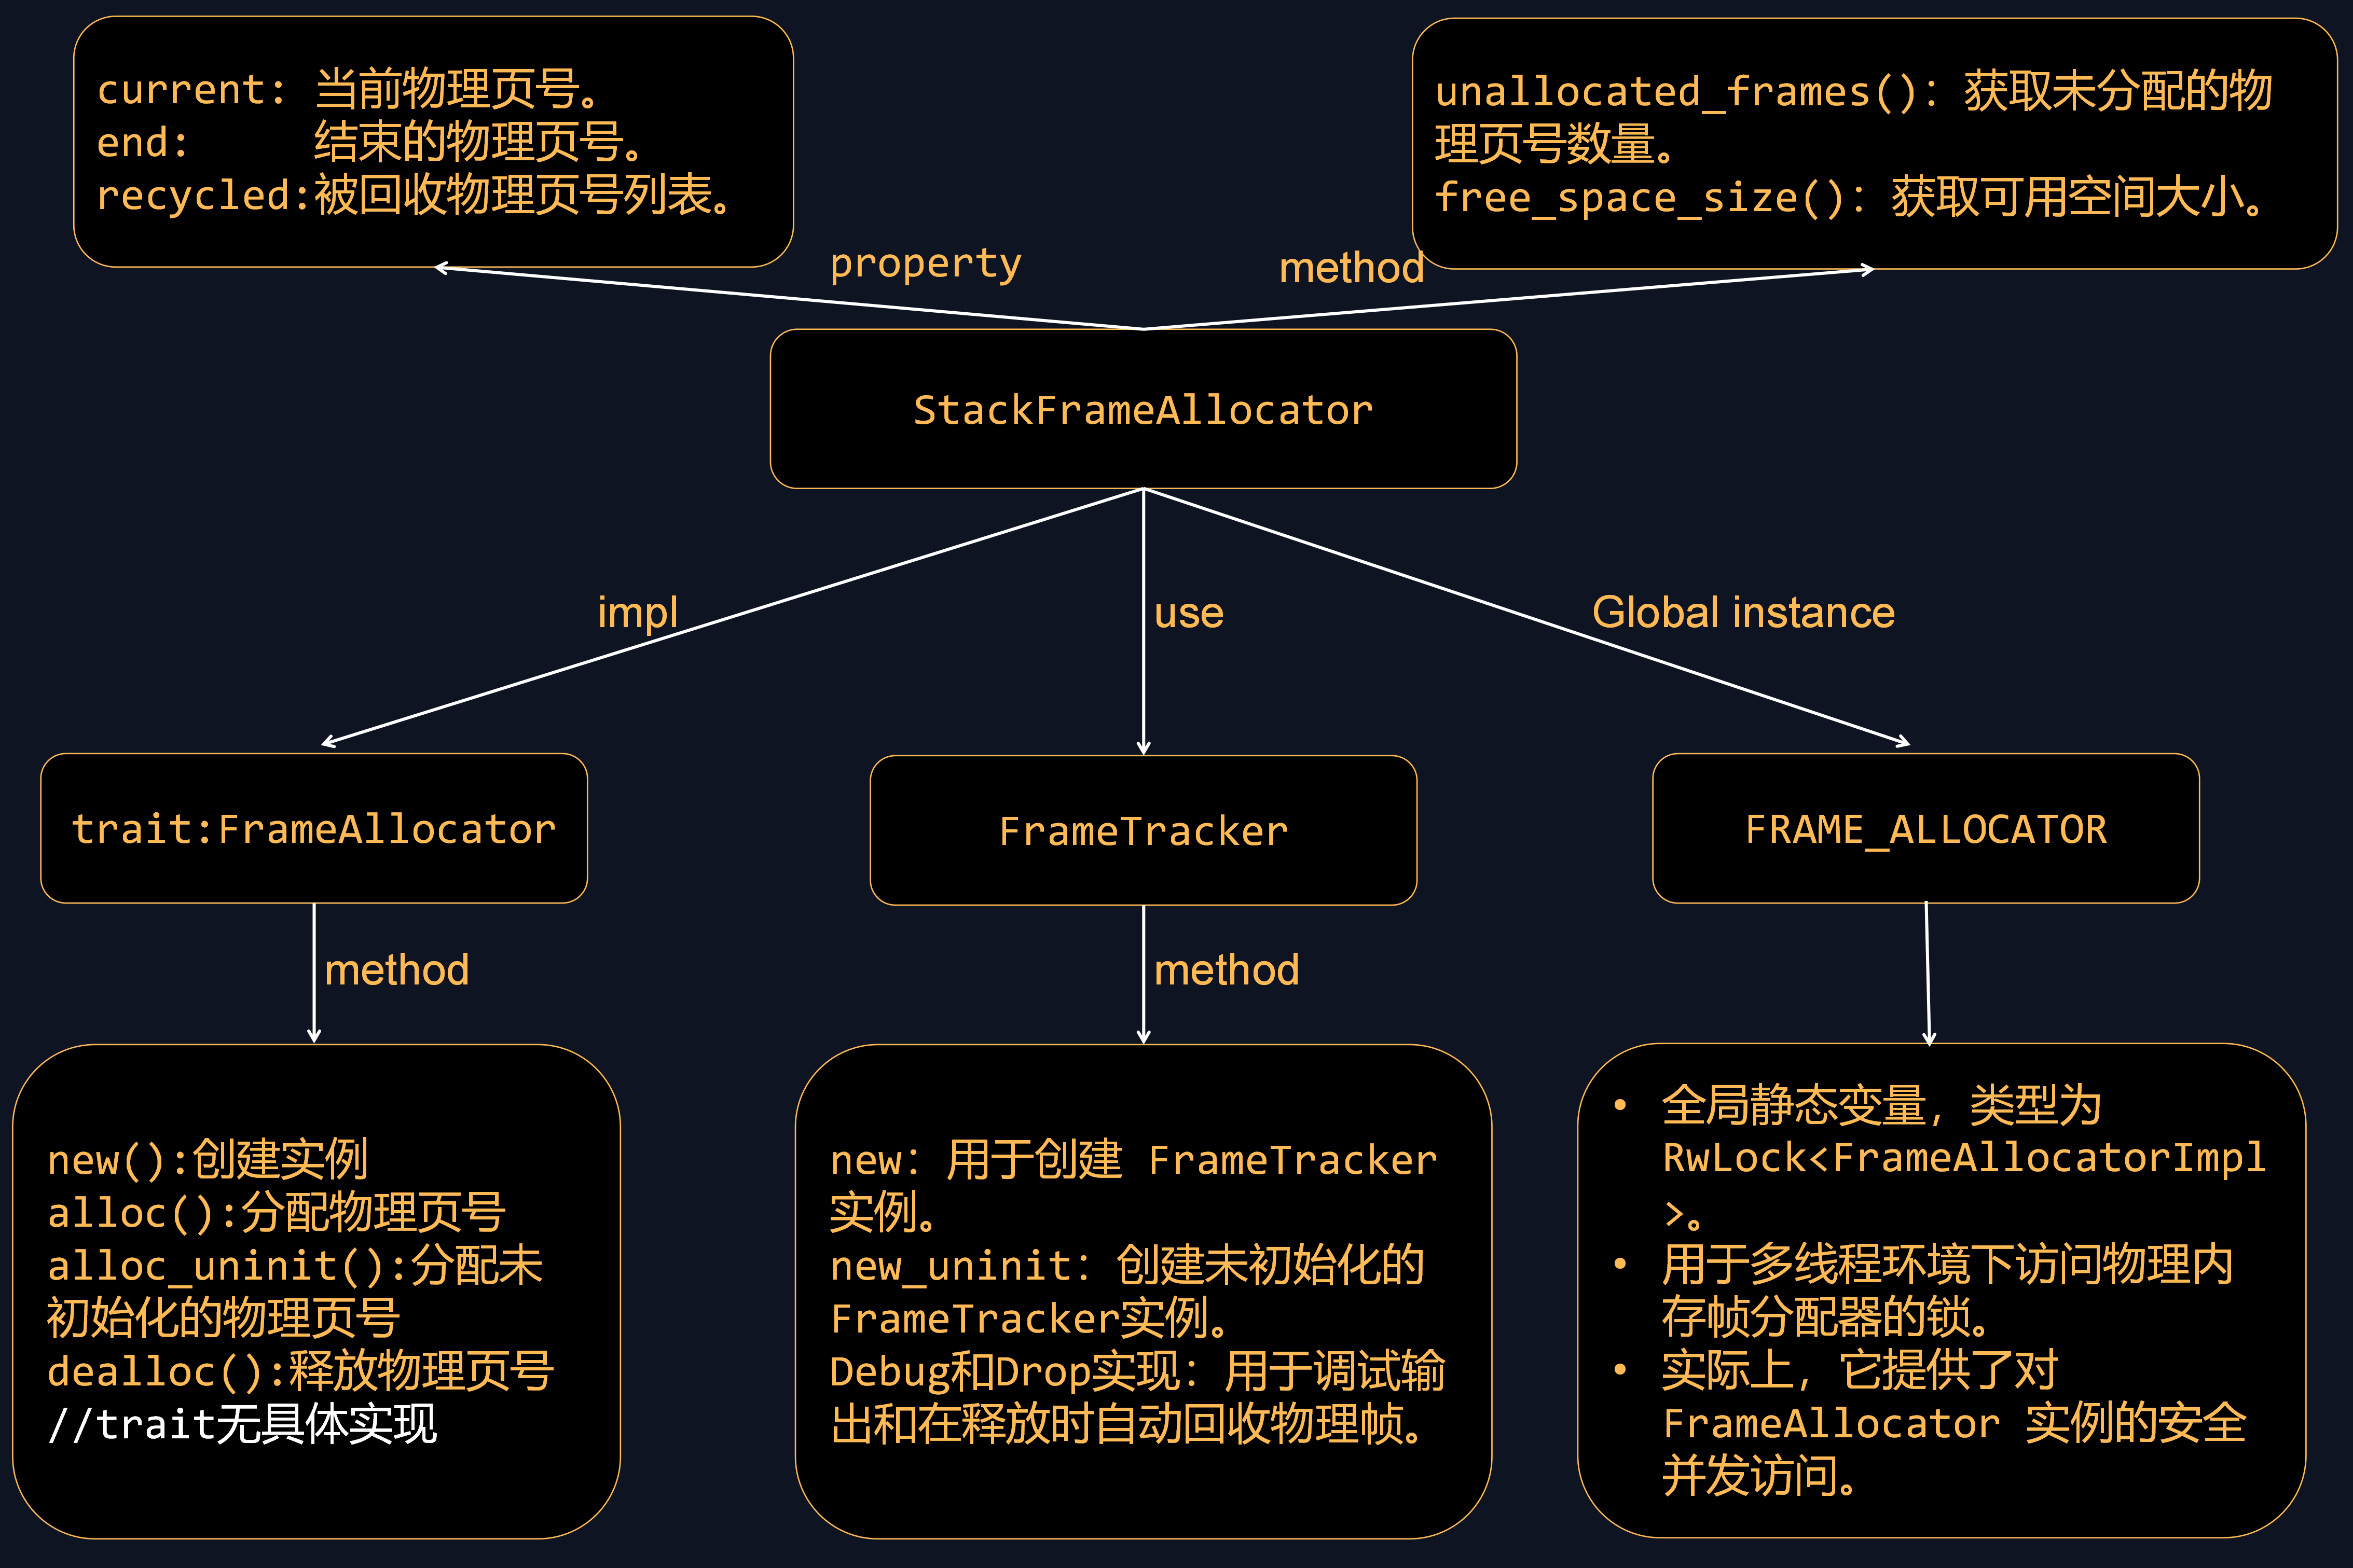
\includegraphics[width=14cm,height=11cm]{figures/04-03-NPUcore中物理内存分配涉及的数据结构.png}
		\caption{NPUcore中物理内存分配涉及的数据结构}
	\end{figure}    
	\justifying  
	\textbf{FrameAllocator trait:}这是一个特性,定义了管理物理内存帧的标准行
	为。它规定了创建、分配、释放物理内存帧的方法。
	
	\textbf{FrameTracker结构体:}用于表示单个物理内存帧的状态,包括物理页号
	(PhysPageNum)以及一些操作方法。这些方法可能涉及物理内存的初始化、
	输出调试信息和回收等,用于创建和管理单个物理内存帧的状态。
	
	\textbf{FRAME\_ALLOCATOR 全局静态变量:}这是用于多线程环境下访问物理内存
	帧分配器的锁。它提供了对 FrameAllocator 实例的安全并发访问。
	
	\textbf{StackFrameAllocator 结构体:}实现了 FrameAllocator 这个
	 trait,用于管理物理内存帧。它采用基于栈的策略来管理物理内存,实现了
	 创建全局变量FRAME\_A
	LLOCATOR 的功能。除此之外,这个结构体还涉及到调用 FrameTracker 中的方法
	,这些方法用于对物理页面进行操作,如初始化、调试输出和回收等。
	
	综上所述,StackFrameAllocator 结构体实现了 FrameAllocator 这个特性,它在
	管理物理内存帧的同时,通过调用 FrameTracker 中的方法对物理页面进行操作。同时,它创建了一个全局变量 FRAME\_ALLOCATOR,
	并提供了线程安全的访问物理内存分配器的机制。
	
	物理内存分配器在计算机操作系统中扮演着非常重要的角色 ,它负责动态地分配和释
	放物理内存资源 ,以确保程序在运行时能够获得足够的物理内存资源 ,并尽可能地
	提高系统的稳定性和性能。
	\begin{figure}[H]
		\centering
		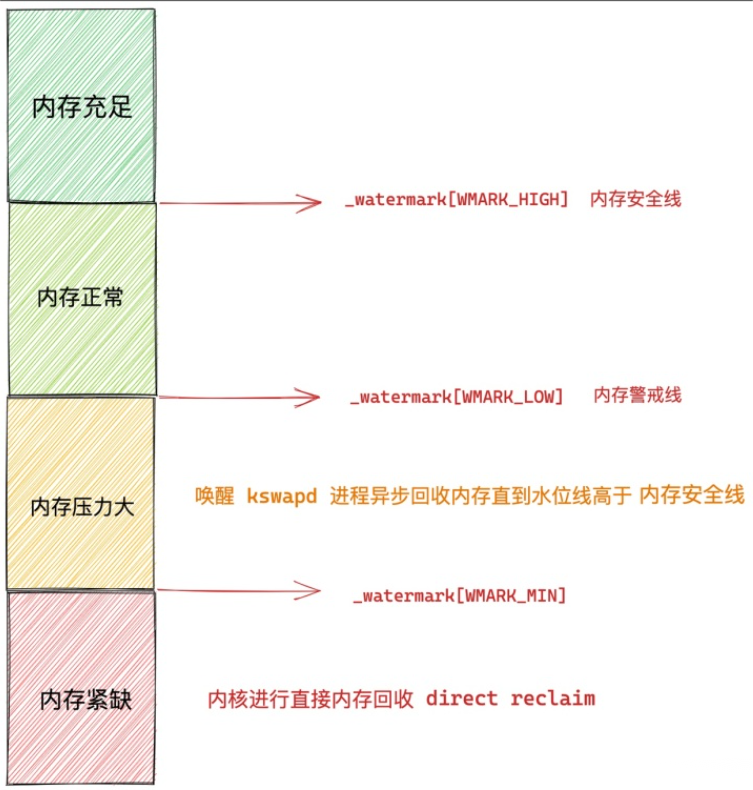
\includegraphics[width=10cm,height=10cm]{figures/04-03-物理内存分配器示意图.png}
		\caption{物理内存分配器示意图}
	\end{figure}   
	物理内存分配器通常包括一个页面置换算法和一个内存映射表。页面置换算法用于在
	内存池中选择要 替换的页面 ,以腾出空间来分配新的页面; 内存映射表用于记录页
	面在内存中的位置和大小 ,以及对应的 虚拟地址。在分配物理内存时 ,物理内存分
	配器会根据页面大小和页面置换算法来决定哪些页面需要被替 换 ,并将新的页面分
	配到内存池中。在程序运 行过程中,如果程序需要的物理内存超过了当前可用的物理
	内存 ,物理内存分配器会根据一定的算法进行 内存释放 ,以腾出物理内存资源,然
	后从内存池中提取所需的物理内存 ,并将其分配给程序运行所需的页面。
	
	\subsection{物理内存空间}
	
	要想有效的管理物理内存 ,首先要清楚我们管理的内存空间范围。在 NPUcore 中 ,
	不同平台上的物理内存空间范围如下:
	
	\begin{lstlisting}[language=Rust]
  // os\src\config.rs
  pub const MEMORY_START:usize = 0x8000_0000;
  #[cfg(all(not(feature = "board_k210"), not(feature = "board_fu740")))]
  pub const MEMORY_END:usize = 0x809e_0000;
  #[cfg(feature = "board_k210")]
  pub const MEMORY_END:usize = 0x8080_0000;
  #[cfg(feature = "board_fu740")]
  pub const MEMORY_ END:usize= 0x9000_0000;
  pub const PAGE_SIZE:usize = 0x1000;
    \end{lstlisting}

	在三个平台上 ,物理内存的起始物理地址 MEMORY\_START 均为  0x80000000 ,单
	个页面大小 PAGE\_SIZE 均为 0x1000 ,即 4096 字节。
	
	在 k210 上 ,我们硬编码整块物理内存的终止物理地址 MEMORY\_END 为 0x80800000 ,这意味着可用 内存大小为  8MiB 。
	
	在 fu740 上 ,   MEMORY\_END 为  0x9000\_0000 ,可用内存大小为 256MiB 。
	
	如果没有 在这两个平台上  (也就是在 qemu 模拟器上)  ,   MEMORY\_END 被设
	置为  0x809e\_0000 ,可用内存大小将  近 10MiB 。	
	\subsection{物理内容分配器初始化}
	
	在编写程序时 ,我们需要将内存分配给自己编写的代码和各种外部库 ,如果在此之
	前未进行正确的内存初始化 ,程序可能会出现各种问题 ,例如内存泄漏、程序崩溃
	等。内存初始化是计算机编程中非常重要的一个步骤 ,用以确保程序在运行时能够正
	确地分配和释放内存,避免不必要的内存浪费和错误它关系到程序能否正确运行以及
	运行的稳定性和可靠性。
	
	内存的初始化中包含物理内存分配器的初始化 ,在这一步骤中 ,使用上文提到的
	物理内存空间来初始 化内存分配器 ,让内存分配器清楚待分配的物理空间范围。
	
	\begin{lstlisting}[language=Rust]
  // os\src\mm\frame_allocator.rs
  pub fn init_frame_allocator(){
    	extern "C" {
	   fn ekernel();
    }
    FRAME_ALLOCATOR .write().init(
    PhysAddr::from(ekernel as usize).ceil(),
    PhysAddr::from(MEMORY_END).floor(),
    );
  }
	\end{lstlisting}
	
	ekernel 即为内核空间的代码和数据存放的末尾 ,此地址即为 MEMORY\_START ,
	从 MEMORY\_START 到 MEMORY\_END ,剩下的空间都将被 frame\_allocator 分
	配使用。
	
	\subsection{物理内存分配器接口}
	在了解了所分配的物理空间范围并完成物理内存分配器的初始化后,我们可以详细了
	解物理内存分配器提供的接口,以及基本的物理内存分配器需要实现哪些功能。
	
	接口描述:物理内存分配器的接口包括一个自身的 new() 方法,以及实现物理页面的
	分配和回收。需要注意的是,这里有一个未初始化的页面分配方法alloc\_uninit(),
	省去初始化操作将会缩短分配时间。
\begin{lstlisting}[language=Rust]
 //os\src\mm\frame_allocator.rs
   trait FrameAllocator {
   fn new()->Self;
   fn alloc(&mut self) -> Option<FrameTracker>;
   unsafe fn alloc_uninit(&mut self) -> Option<FrameTracker>;
   fn dealloc(&mut self,ppn:PhysPageNum);
  }
\end{lstlisting}
    
    RAII与FrameTracker在前文介绍地址空间时提到,FrameTracker绑定了每个物理页面
    作为物理页面追踪器,将物理页面追踪器映射到虚拟页面有利于RAII和页面查找;RAII
    指的是FrameTracker与物理页面具有相同的生命周期,在获取物理页面构建FrameTrac
    ker时会将物理页面初始化,在drop FrameTracker时也会自动回收物理页面。
    
    \begin{lstlisting}[language=Rust]
 //os\src\mm\frame_allocator.rs
   pub struct FrameTracker {
     pub ppn:PhysPageNum,
   }
 ///RAII phantom for physical pages
    \end{lstlisting}

    new方法具体实现在new()方法中,获取物理页面号后,通过get\_dwords\_array()获
    取64字节的数组,逐个元素赋零以实现页面的初始化(清零)。
    
\begin{lstlisting}[language=Rust]
 pub fn new(ppn:PhysPageNum) -> Self {
 // page cleaning
  let dwords_array = ppn.get_dwords_array();
  for i in dwords_array {
	  *i = 0;
	}
  Self {ppn}
}
\end{lstlisting}
    
    new\_uninit()提高性能原因:循环赋零会产生时间开销。为了应对一些情况下不需
    要对页面进行清零操作的情况(比如上一节介绍的COW处理,在申请到新页面时直接进
    行完全拷贝),提供了new\_uninit()方法,它不执行清零操作,直接返回由物理页面
    号构造的FrameTracker实例。
    
    \begin{lstlisting}[language=Rust]
 pub unsafe fn new_uninit(ppn:PhysPageNum)->Self {
    Self {ppn}
  }
    \end{lstlisting}

正是在FrameTracker提供了new\_uninit的方法,才在上层的FrameAllocator中支持了
alloc\_uninit。

	\subsection{全局物理内存分配器}
	
	全局物理内存分配器是一种用于分配和释放物理内存的机制 ,用于解决程序在运行时
	的内存分配 和释放问题。在计算机程序中 ,内存分配和释放通常是由不同的进程或
	线程进行的 ,这可能会导致内存泄 漏和其他问题。
	
	如果没有全局物理内存分配器 ,每个进程或线程都需要自己管理内存分配和释放 ,
	那么可能会出现以 下问题:
	
	\textbf{内存泄漏 :}当程序在分配内存时 ,如果未能正确释放内存 ,则可能会
	导致内存泄漏。这会导致程序占 用的内存不断增加 ,最终导致程序崩溃或拒绝服务。
	
	\textbf{内存分配异常 :}如果进程或线程需要分配的内存大小超过了系统可用的内存大小
	 ,则可能会导致内存 分配异常。这可能会导致程序崩溃或拒绝服务。
	
	\textbf{内存分配和释放的不稳定性 :}每个进程或线程都需要自己管理内存分配和
	释放,这可能会导致内存分 配和释放的不稳定性。例如 ,某个进程或线程可能会
	在释放内存后不久就重新分配内存 ,从而导致内存泄漏或其他问题。
	
	为了解决这些问题 ,我们需要一个全局的物理内存分配器来负责管理程序运行时的物
	理内存分 配和释放。全局物理内存分配器可以确保内存分配和释放的稳定性和可靠性
	 ,减少内存泄漏和其他问题的 发生。此外 ,全局物理内存分配器还可以提高程序的
	 性能和吞吐量 ,因为内存分配和释放不再由不同的进 程或线程单独管理 ,而是由
	 一个统一的内存管理机制来负责。
	
	接下来我们深入 NPUcore 内部 ,探究一下 NPUcore 是如何实现全局物理内存分配
	器的。
	
	首先创建一下  StackFrameAllocator 的全局实例  FRAME\_ALLOCATOR  :
\begin{lstlisting}[language=Rust]
  // os\src\mm\frame_allocator.rs
    type FrameAllocatorImpl = StackFrameAllocator;
    lazy_static!{
      pub static ref FRAME_ALLOCATOR:RwLock<FrameAllocatorImpl>=
    RwLock::new(FrameAllocatorImpl::new());
    }
\end{lstlisting}

	这里我们使用  RwLock\textless T\textgreater 来包裹栈式物理页帧分配器 ,
	加上一层读写锁。每次对该分配器进行操作之前 ,我们都需要先通过  FRAME\_ALLOCATOR .write() 拿到分配器的写权限 ,以保证排他性。
	
	公开给其他内核模块调用的分配/回收物理页帧的接口为 :
\begin{lstlisting}[language=Rust]
  // os\src\mm\frame_allocator.rs
  pub fn frame_alloc() -> Option<Arc<FrameTracker>> {
    FRAME_ALLOCATOR
   .write().alloc().map(|frame_tracker|Arc::new(frame_tracker))
  }
  pub unsafe fn frame_alloc_uninit() -> Option<Arc<FrameTracker>> {
    FRAME_ALLOCATOR
   .write().alloc_uninit().map(|frame_tracker|Arc::new(frame_tracker))
  }
  pub fn frame_dealloc(ppn:PhysPageNum) {
    FRAME_ALLOCATOR.write().dealloc(ppn);
  }
\end{lstlisting}

	alloc 申请来的 frame\_tracker 用 Arc 包裹实现自动引用计数再返回。在 FrameTracker 被Drop的时候 ,会调用 frame\_dealloc 方法。
\begin{lstlisting}[language=Rust]
  // os\src\mm\frame_allocator.rs
  impl Drop for FrameTracker{
    //Automatically recycle the physical frame when
    fn drop(&mut self) {
      // println!("do drop at {}", self.ppn.0);
      frame_dealloc(self.ppn);
    }
   }
\end{lstlisting}

	这样就做到了当一个  FrameTracker 实例被回收的时候 ,它的  drop 方法会自动
	被编译器调用 ,通 过之前实现的  frame\_dealloc ,进一步调用 StackFrameAllocator 的 dealloc ,即可将它控制的物理 页帧回收以供后续使用
	。
	
	通过全局物理内存分配器的包装 ,在内核其他模块的视角下 ,  申请一个物理页面
	会返回 FrameTracker ,当 FrameTracker 生命期结束,物理页面也就被自动回收
	 ,体现了 RAII 的思想。
	\section{内存分配办法}
	全局物理内存分配器提供给内核其他模块申请物理内存的统一方法 ,而物理内存分配
	方法的具体实现 在内存分配器中。接下来让我们深入物理内存分配器内部,来探究一
	下在物理内存分配器内部是如何实现 物理内存分配的。
	
	在物理内存分配方法中 ,一种常用并且简单有效的管理策略为栈式内存管理。  它
	不但存取速度快 ,而 且数据存取操作十分简单 ,表示操作也比较容易 ,存储空间
	可用性较大 ,  占用存储空间也小,有很强的 数据抽象能力 ,程序代码表示简洁
	,工作方便。
	
	栈式管理 ,数据的读写只能从一端进行 ,遵循后进先出的原则 ,与堆放木柴一样 ,最后放进去的木柴 在上面 ,是下次最先取出的一块木柴。
	
	NPUcore 使用的正是栈式的内存管理策略 ,下面我们将以 NPUcore 的具体实现为
	例 ,来介绍物理内 存分配方法。
	\subsection{栈式内存管理}
	首先用一个结构体来记录空闲的物理页面 :
	\begin{lstlisting}[language=Rust]
	pub struct StackFrameAllocator {
        current:usize,     
        end:usize,         
        recycled:Vec<usize>,}
	\end{lstlisting}
	为这个 StackFrameAllocator 实现 FrameAllocator 接口 ,   new 方法将空闲
	内存区间两端均设为 0,然后创建一个新的向量。
\begin{lstlisting}[language=Rust]
  // os\src\mm\frame_allocator .rs
  impl FrameAllocator for StackFrameAllocator {
    fn new() -> Self {
	  Self {
		  current:0,
		  end:0,
		  recycled:Vec::new(),
	       }
	 }
    }
\end{lstlisting}
	
	在它真正被使用起来之前 ,需要调用 StackFrameAllocator 的  init 方法将自身的  [current,end) 初始化为可用物理页号区间。
	
	用结束物理页号减去起始物理页号得到剩余有多少物理页面。在内核运行时输出的 last {} Physical Frames, 就是起源于这里 ,输出还有多少空闲页面。这里还
	用了向量的 reserve 方 法来预留出足够的空间 ,避免在运行中不断的重新分配。
	该方法的方法签名为“pub fn reserve(\&mut self, additional: usize)”,用于为 Vec \textless T\textgreater 预留至少 additional 个元
	素的容量。调用reserve 后, Vec 的容量将大于或等于 self.len() + additional
	。如果当前容量已经足够,该方法则不执行任何操作。
	
\begin{lstlisting}[language=Rust]
  // os\src\mm\frame_allocator.rs
  impl StackFrameAllocator{
  pub fn init(&mut self, l:PhysPageNum, r:PhysPageNum) {
    self.current = l.0;
    self.end = r.0;
    let last_frames = self.end - self.current;
    self.recycled.reserve(last_frames);
    println !("last {} Physical Frames.", last_frames);
  }
  pub fn unallocated_frames(&self) -> usize {
    self.recycled.len() + self.end - self.current
  }
  pub fn free_space_size(&self) -> usize {
    self.unallocated_frames() * PAGE_SIZE
  }
  }
\end{lstlisting}
	
	unallocated\_frames 用于计算未被分配的页面数量 ,为 recycled 中的空闲页面
	和整块的空闲内存 页面数量之和。   free\_space\_size 计算空闲空间的大小 ,
	只需空闲页面的数量乘页面大小。
	\subsection{物理页帧分配}
	核心为物理页帧的分配和回收 ,先看物理页帧的分配 :
	
	在分配  alloc 的时候 ,首先会检查栈  recycled 内有没有之前回收的物理页号 
	,如果有的话弹出栈顶 ,使用  into 方法将  usize 转换成了物理页号  PhysPageNum ,构造 frame\_tracker 返回。否则检 查 current ==  end ,若
	相等则表示内存耗尽 ,没有空闲页面 ,返回 None 。
\begin{lstlisting}[language=Rust]
  // os\src\mm\frame_allocator.rs
  impl FrameAllocator for StackFrameAllocator {
    fn alloc(&mut self) -> Option<FrameTracker> {
	if let Some(ppn) = self.recycled.pop() {
	  let frame_tracker = FrameTracker::new(ppn.into());
	  log::trace!("[frame_alloc] {:?}",frame_tracker);
	  Some(frame_tracker)
	} else if self.current == self.end {
	  None
	} else {
	  self.current += 1;
	  let frame_tracker = FrameTracker::new((self.current - 1).into());
	  log::trace!("[frame_alloc]{:?}",frame_tracker);
	  Some(frame_tracker)
	}
   }
  }
\end{lstlisting}
	
	若不等说明之前从未分配过的物理页号区间还有剩余 ,可以在 [  current ,  end
	 ) 上进行分配 ,我们 分配它的左端点  current  (即从低地址向高地址分配)  
	 ,同时将管理器内部维护的  current 加  1 代表current 已被分配了。  同样将
	   usize 转换成了物理页号 ,构造 frame\_tracker 返回。
	
	之前提到过 FrameAllocator 有一个不初始化分配方法 alloc\_uninit ,我们看一
	下二者的不同 :
	\begin{figure}[H]
	  \centering
	  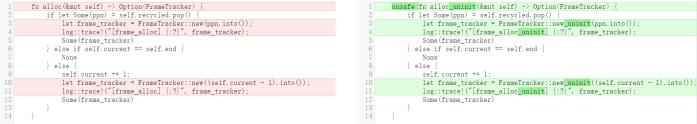
\includegraphics[width=14cm,height=3cm]{figures/04-03-alloc与alloc_uninit对比图.png}
	  \caption{alloc与alloc\_uninit对比图}
	\end{figure}
	
	其实也就是在 FrameTracker::new 的时候不同 ,在 alloc 中使用的是 FrameTracker::new 这个有初 始化的方法 ,在 alloc\_uninit 中使用的是 FrameTracker::new\_uninit 这个不初始化的方法。
	\subsection{物理页帧回收}
	物理页帧的回收是整个内存管理中一个重要的环节,它负责释放不再被使用的页面以
	供后续分配使用。让我们来看一下物理页面的回收机制以及其实现的过程。
	
\begin{lstlisting}[language=Rust]
  // os\src\mm\frame_allocator.rs
  // Deallocate a physical page
  fn dealloc(&mut self,ppn:PhysPageNum){
    log::trace!("[frame_dealloc] {:?}", ppn);
    let ppn = ppn.0;
    // validity check, note that this should be unnecessary for RELEASE build and it
    if option_env!("MODE") == Some("debug") && ppn >= self .current
    self .recycled.iter().find(|&v|*v == ppn).is_some()
    {
    	panic!("Frame ppn={:#x} has not been allocated!",ppn);
    }
    // recycle
    self.recycled.push(ppn);
}
\end{lstlisting}
  
  在这个回收的过程中,首先记录了将要回收的物理页面ppn,然后在调试模式下进行了有效
  性检查,以确保被释放的物理页面确实已经被分配过,防止程序在运行时因未分配的页面
  进行回收而出现问题。
  
  这个有效性检查使用了recycled.iter().find()方法,耗时较多,这也是为何在构建
  RELEASE版本时不必执行该检查的原因。对于发布版本来说,已经经过充分测试,假设不
  会出现未分配页面回收的情况。
  
  实际的页面回收机制非常简单,它仅将要回收的页面号ppn压入回收页面的recycled向量
  中。这个向量用于存储可供重新分配的物理页面。物理页面的回收是内存管理中重要的一
  环,通过这个机制,系统可以及时释放不再使用的页面,并通过有效性检查和回收流程来
  确保内存的正确性和可靠性。
%\end{document}
